\section{Gain saturation}

Gain saturation describes a phenomenon that occurs when the active region of a laser is unable to maintain its gain as intercavitiy power increases. The gain of a laser is proportional to the population of excited carriers in the active region. As the intercavitiy power rises, the stimulated emission rate of photons increases, depleting the population of excited carriers. If the rate of stimulated emission exceeds the rate at which carriers are being excited, the population of excited carriers diminishes and therefore decreasing the gain, i.e. the gain gets saturated. The gain saturation in semiconductor laser is a dynamic process, due to short carrier lifetimes and rapid recombination processes on the order of picoseconds to nanoseconds. Whereas for ion-doped solid state laser (e.g. Ti:Sapphire lasers) the gain saturation is not dynamic, since the relevant time scales are on the order of milliseconds.

To study this behaviour, one measures the nonlinear behaviour of the reflectivity for an increasing amount of probe fluence, as can be seen in \cref{fig:gainSat}. To quantify this behaviour and gain some macroscopic parameters, a model based on the saturation of the absorber in a SESAM can be fitted to the data \cite{Haiml2004OpticalAbsorbers}. 

\begin{equation}
    \centering
    R(F)=R_{ns} \frac{F_{sat}}{F} \ln\left\{1 + \frac{R_{ss}}{R_{ns}} \left[\exp{ \left(\frac{F}{F_{sat}}\right) } - 1\right]\right\} \exp{\left(-\frac{F}{F_2}\right)}
    \label{eq:model}
\end{equation}

The parameters from \cref{eq:model} are the saturation fluence $F_{sat}$, the small signal reflectivity $R_{ss}$, the nonsaturable reflectivity $R_{ns}$ and the rollover parameter $F_{2}$.

The saturation fluence $F_{sat}$ is the fluence at which the reflectivity reduces to $1/e$ of its maximum. It also represents the point at which the population inversion inside the active region becomes saturated, therefore it is closely tied to the material properties of the active region.

The small signal reflectivity $R_{ss}$ refers to the reflectivity at low probe fluence, where the gain is not significantly saturated. In this regime nonlinear effects are minimal and the reflectivity can be considered to be in the linear regime and the small signal gain can be calculated as $g_{ss}=R_{ss}-100\%$.

The nonsaturable reflectivity $R_{ns}$ arises from absorption and scattering at impurities and interfaces inside the VECSEL structure. This limits the maximum performance of the VECSEL, thus reducing defect density during the growing process is important. Since this effect is associated with imperfection and reflection inside the structure it remains constant for different probe fluences. 

The rollover parameter $F_2$ describes further absorption from two photon absorption or higher order effects resulting in a strong decrease in the reflectivity at high fluences.

\Cref{fig:gainSat} shows the key parameters and the fitted model with and without accounting for the rollover for a measurement of a VECSEL with an integrated pump DBR.


\begin{figure}[ht]
    \centering
    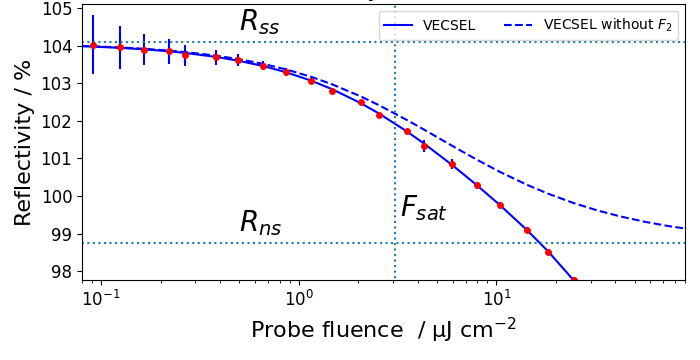
\includegraphics[width=12cm]{images/gainSat.png}
    \caption{Nonlinear reflectivity measurement for a VECSEL with integrated pump DBR and diamond heat spreader versus probe fluence. The data is shown with the fitted model utilizing \cref{eq:model} and the same model without the rollover parameter $F_2$. Additionally the different parameters $R_{ss}$, $R_{ns}$ and $F_{sat}$ are visualized.}
    \label{fig:gainSat}
\end{figure}